\documentclass{article}

\usepackage{graphicx}
\usepackage{tikz}
\usepackage{tikzsymbols}
\usetikzlibrary{calc,patterns,shapes.geometric}
\pagestyle{empty}
\usepackage[margin=0pt]{geometry}
\geometry{papersize={14in,12in}}

\def\centerarc[#1](#2)(#3:#4:#5){\draw[#1] ($(#2)+({#5*cos(#3)},{#5*sin(#3)})$) arc (#3:#4:#5);}

\begin{document}
	\begin{figure}
		\centering
		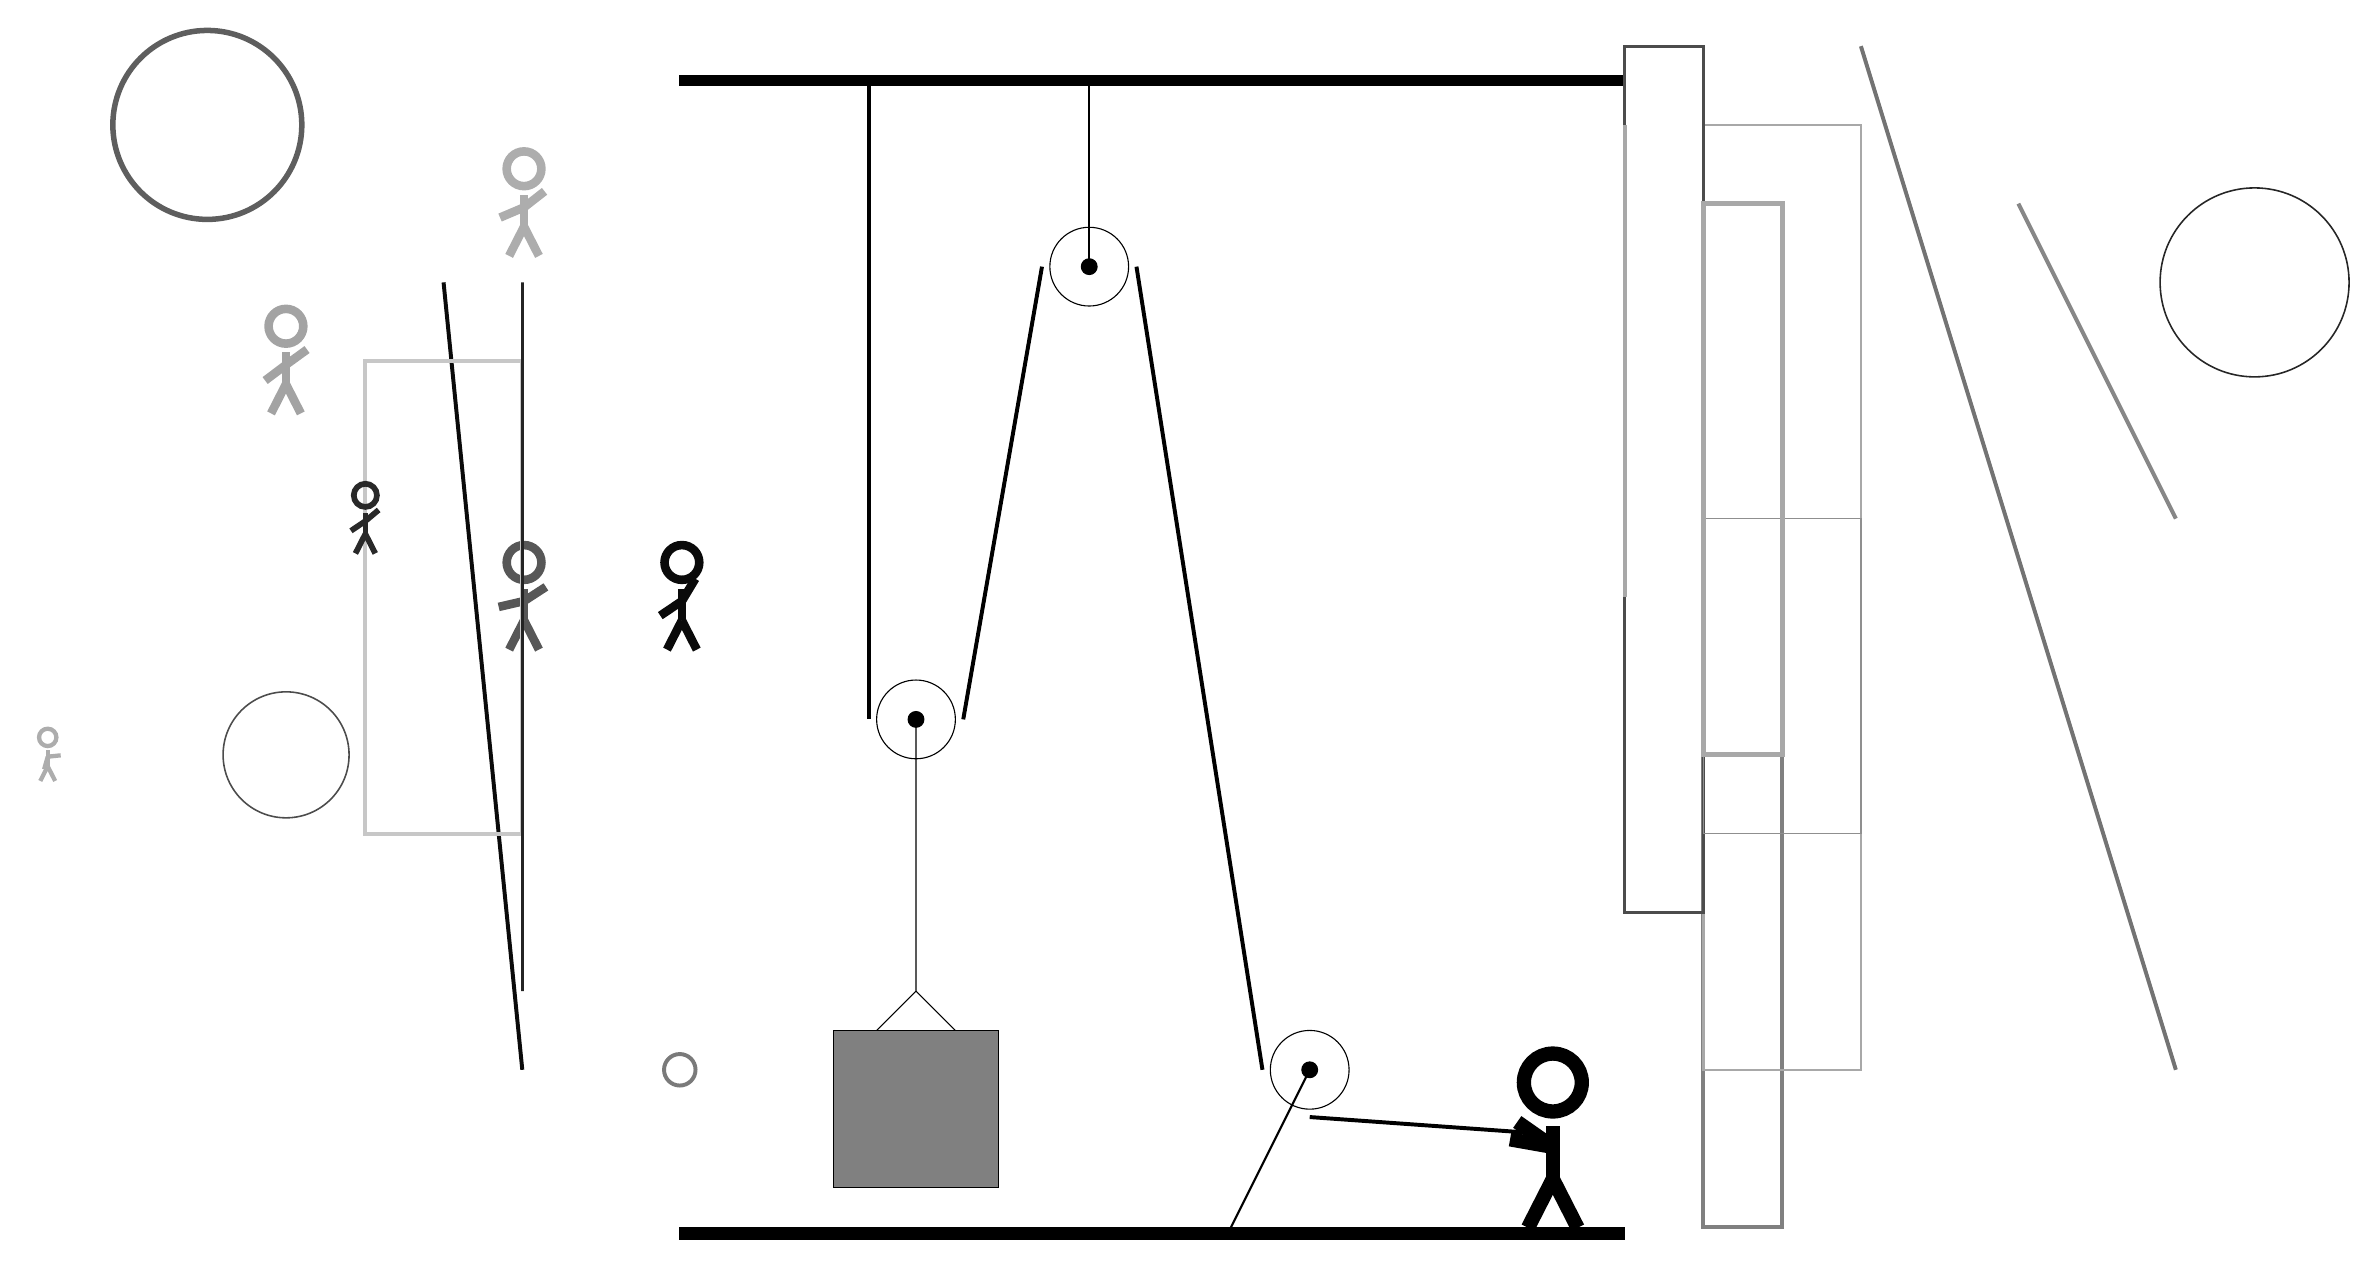
\begin{tikzpicture}
			%%%%% START %%%%%
			
			\draw[fill=black] (-2, 11.5) rectangle (10, 11.625);
			
			\draw (3.2, 9.2) circle (0.5);
			\draw[fill=black] (3.2, 9.2) circle (0.1);
			\draw[thick] (3.2, 9.2) -- (3.2, 11.5);
			
			\draw (6, -1) circle (0.5);
			\draw[fill=black] (6, -1) circle (0.1);
			\draw[thick] (6, -1) -- (5, -3);
			
			\draw (1, 3.45) circle (0.5);
			\draw[fill=black] (1, 3.45) circle (0.1);
			
			\draw[line width=0.5mm, color=black!50] (11, 3) rectangle (12, -3);
			
			\draw[line width=0.5mm, color=black!96](-5, 9) -- (-4, -1);
			\draw [line width=0.7mm, color=black!63](-8, 11) circle (1.2);
			\draw[line width=0.3mm, color=black!34] (11, 11) rectangle (13, -1);
			\node[line width=0.6mm, color=black!96] at (-2, 5) {\Strichmaxerl[6][34][59]};
			\draw[line width=0.4mm, color=black!70] (11, 12) rectangle (10, 1);
			\draw[line width=0.2mm, color=black!44] (11, 6) rectangle (13, 2);
			\node[line width=0.4mm, color=black!32] at (-10, 3) {\Strichmaxerl[3][74][6]};
			\draw[line width=0.5mm, color=black!47](15, 10) -- (17, 6);
			\draw [line width=0.2mm, color=black!70](-7, 3) circle (0.8);
			
			\draw [line width=0.2mm, color=black!85](18, 9) circle (1.2);
			
			\draw[line width=0.6mm, color=black!34] (11, 10) rectangle (12, 3);
			\draw [line width=0.5mm, color=black!52](-2, -1) circle (0.2);
			\draw[line width=0.5mm, color=black!34](10, 11) -- (10, 5);
			\node[line width=0.2mm, color=black!36] at (-7, 8) {\Strichmaxerl[6][37][36]};
			\draw[line width=0.5mm, color=black!55](13, 12) -- (17, -1);
			
			\node[line width=0.5mm, color=black!66] at (-4, 5) {\Strichmaxerl[6][13][33]};
			\draw[line width=0.5mm, color=black!22] (-4, 2) rectangle (-6, 8);
			\node[line width=0.5mm, color=black!84] at (-6, 6) {\Strichmaxerl[4][34][40]};
			\node[line width=0.7mm, color=black!32] at (-4, 10) {\Strichmaxerl[6][23][38]};
			\draw[line width=0.4mm, color=black!86] (-4, 0) rectangle (-4, 9);
			
			\draw (1, 3.45) -- (1, 0.0) -- (0.5, -0.5);
			\draw (1, 0.0) -- (1.5, -0.5);
			\draw[fill=black!50] (-0.05, -0.5) rectangle (2.05, -2.5);
			
			\draw[line width=0.5mm] (0.4, 11.5) -- (0.4, 3.45);
			\centerarc[line width=0.5mm](1, 3.45)(180:360:0.6);
			\draw[line width=0.5mm](1.6, 3.45) -- (2.6, 9.2);
			\centerarc[line width=0.5mm](3.2, 9.2)(0:180:0.6);
			\draw[line width=0.5mm](3.8, 9.2) -- (5.4, -1);
			\centerarc[line width=0.5mm](6, -1)(180:270:0.6);
			\draw[line width=0.5mm](6, -1.6) -- (8.8, -1.8);
			
			\node at (9, -1.9) {\Strichmaxerl[10][-35][170]};
			
			\draw[fill=black] (-2, -3) rectangle (10, -3.15);
			
			%%%%% END %%%%%
		\end{tikzpicture}
	\end{figure}	
\end{document}